% !TEX TS-program = pdflatex
% !TEX encoding = UTF-8 Unicode

% This is a simple template for a LaTeX document using the "article" class.
% See "book", "report", "letter" for other types of document.

\documentclass[12pt]{article} % use larger type; default would be 10pt

\usepackage[utf8]{inputenc} % set input encoding (not needed with XeLaTeX)

%%% Examples of Article customizations
% These packages are optional, depending whether you want the features they provide.
% See the LaTeX Companion or other references for full information.

%%% PAGE DIMENSIONS
\usepackage{geometry} % to change the page dimensions
\geometry{a4paper} % or letterpaper (US) or a5paper or....
% \geometry{margin=2in} % for example, change the margins to 2 inches all round
% \geometry{landscape} % set up the page for landscape
%   read geometry.pdf for detailed page layout information

\usepackage{graphicx} % support the \includegraphics command and options

% \usepackage[parfill]{parskip} % Activate to begin paragraphs with an empty line rather than an indent

%%% PACKAGES
\usepackage{booktabs} % for much better looking tables
\usepackage{array} % for better arrays (eg matrices) in maths
\usepackage{paralist} % very flexible & customisable lists (eg. enumerate/itemize, etc.)
\usepackage{verbatim} % adds environment for commenting out blocks of text & for better verbatim
\usepackage{subfig} % make it possible to include more than one captioned figure/table in a single float
% These packages are all incorporated in the memoir class to one degree or another...

%%% HEADERS & FOOTERS
\usepackage{fancyhdr} % This should be set AFTER setting up the page geometry
\pagestyle{fancy} % options: empty , plain , fancy
\renewcommand{\headrulewidth}{0pt} % customise the layout...
\lhead{}\chead{}\rhead{}
\lfoot{}\cfoot{\thepage}\rfoot{}

%%% SECTION TITLE APPEARANCE
\usepackage{sectsty}
\allsectionsfont{\sffamily\mdseries\upshape} % (See the fntguide.pdf for font help)
% (This matches ConTeXt defaults)

%%% ToC (table of contents) APPEARANCE
\usepackage[nottoc,notlof,notlot]{tocbibind} % Put the bibliography in the ToC
\usepackage[titles,subfigure]{tocloft} % Alter the style of the Table of Contents
\renewcommand{\cftsecfont}{\rmfamily\mdseries\upshape}
\renewcommand{\cftsecpagefont}{\rmfamily\mdseries\upshape} % No bold!

%immagini
\usepackage{graphicx}
\graphicspath{ {./images/} }

%font sezioni ecc
\usepackage{titlesec}

\titleformat{\section} {\normalfont\large\bfseries\centering}{\thesection}{1em}{}
\titleformat{\subsection} {\normalfont\large}{\thesubsection}{1em}{}
\titleformat{\subsubsection} {\normalfont\normalsize}{\thesubsubsection}{1em}{}
\titleformat{\paragraph}[runin] {\normalfont\normalsize}{\theparagraph}{1em}{}
\titleformat{\subparagraph}[runin] {\normalfont\normalsize}{\thesubparagraph}{1em}{}

\pretolerance=10000
\tolerance=2000 
\emergencystretch=10pt

%%% END Article customizations

%%% The "real" document content comes below...



 



\begin{document}


\begin{center}
       \vspace*{1cm}
 
       \Large{\textbf{Progetto Esame Microelettronica - Modulo A}}
 
       \vspace{0.5cm}
        Realizzazione Full adder a 4 bit
 
       \vspace{1.5cm}
 
       Alessio Capello\\
 
       Matricola 3811634
 
       \vspace{1.5cm}
 
 
       Università degli studi di Genova\\
       Ingegneria elettronica\\
       Data   
\end{center}
\clearpage

\tableofcontents

\clearpage

\section{Obiettivi del progetto}
Il progetto ha come scopo la realizzazione di un full-adder a 1 bit con tecnologia MOS 0.12 $\mu$m e logica TSPC. \\
Il circuito sarà quindi pilotato da 3 ingressi($a_{0},b_{0}, c_{0}$) relativi ai segnali logici e un ingresso dedicato al clock (il segnale $\phi$).
Le uscite del circuito sono i segnali di $SUM$ e $CARRY$.\\
Successivamente si dovranno connettere 4 full-adder a 1 bit precedentemente descritti per comporre un full-adder a 4 bit.
Il full adder risultante avrà quindi due ingressi a 4 bit (per il dato $a$ ed il dato $b$) e un ingresso a un bit per il carry $c$. Anche in quest'ultimo caso sarà presente il segnale di clock come ingresso.
\subsection{Specifiche del Progetto}
Le specifiche del circuito definiscono:
\begin{itemize}
\item Tecnologia MOS 0.12 $\mu$m con logica TSPC
\item Un'alimentazione  pari a $1.2V$ 
\item Una frequenza di lavoro (del clock) di $2GHz$. 
\item Il carico da pilotare è una capacità di $100fF$.
\item Il layout proposto dovrà avere un'altezza massima di 68$\lambda$.
\end{itemize}

\section{Cenni teorici}
La logica TSPC (true single phase clock) è un tipo di struttura circuitale utilizzata per progettare circuiti temporizzati da un singolo segnale di clock $\phi$. \\
Si compone di due parti principali: una logica statica (di tipo N) per l'elaborazione dei bit e un latch di uscita.
Il circuito lavora in due fasi distinte:
\begin{itemize}
\item Quando il segnale di clock ha valore basso il circuito è in \textbf{fase di precarica}.
\item Quando il segnale di clock ha valore alto il circuito è in \textbf{fase di valutazione}. Le uscite possono essere considerate corrette solamente in questa fase (terminati i transitori).
\end{itemize}
La logica N ha come scopo di connettere l'uscita a massa (quindi di scaricare, quando la logica lo prevede, le capacità precedentemente caricate).

\clearpage
\section{Dimensionamento}
Per dimensionare il circuito (ovvero stabilire i rapporti W/L dei singoli transistor) sono state considerate le specifiche relative alla frequenza di funzionamento e al carico. Questi infatti sono i vincoli determinati dalle caratteristiche dell'ultimo stadio, che a cascata si riverberano su quelli precedenti. 
Per questo motivo, il dimensionamento prevede di stabilire per primo il fattore di forma dello stadio finale.
Le dimensioni del transistor sono state ottenute considerando la formula seguente:

\begin{equation} 
\frac{W}{L}=\frac{2CV_{dd}}{\tau \mu_{n}C_{ox}(V_{gs}-V_{th})^2}
\end{equation}
Dove:

\begin{itemize}
\item $V_{gs}$ = $1.20V$ 
\item $C$ = $100$ $fF$ 
\item $\tau$ = $250$ $ps$
\item $\mu_{n}$ = $0.06$ $m^2/Vs$  
\item $C_{ox}$ = $0.01725$ $fF/m^2$ 
\item $V_{gs} - V_{th}$ = $0.8V$ 
\end{itemize}


Ottenuto il rapporto $W/L$ per arrivare alle dimensioni esatte del transistor si è considerata una lunghezza di canale pari a 120nm. La larghezza del transistor deve essere un multiplo intero della lunghezza del canale, valori ottenuti relativi al terzo stadio sono quindi:

\begin{itemize}
\item $W/L = 1.4486 => 2$  Per arrotondamento all'intero successivo.
\item $W_{n} = 240 nm$ Moltiplicando il rapporto W/L per la lunghezza di canale.
\item $W_{n} = 720 nm$ Considerando che la mobilità dei portatori positivi è inferiore a quella dei portatori negativi, è necessario aumentare il rapporto W/L di 3 volte per avere le stesse performance.
\end{itemize}

Essendo ora note le caratteristiche del terzo stadio, si può procedere a dimensionare gli stadi precedenti.
Si calcola la capacità vista dai transistor del secondo stadio (ovvero la capacità d'ingresso dei transistor del terzo stadio) con la seguente formula:
\begin{equation} 
C_{G}= (C_{ox}W_{N}L) + (C_{ox}W_{P}L)
\end{equation}
Si ottiene una capacità pari a $2.93$ $fF$. Con una grandezza così piccola in gioco è sufficiente un transistor a dimensione minima (quindi con $W/L =1$) per pilotare i gate del terzo stadio.
Una considerazione analoga può essere fatta per i transitor del primo stadio. Si ottiene quindi che tutti i transistor ad eccezione di quelli del terzo stadio saranno a dimensione minima:

\begin{itemize}
\item $W_{n} = 120 nm$ Dimensione minima :  $W/L = 1$
\item $W_{p} = 360 nm$ Dimensione minima per un transistor P
\end{itemize}

\section{Realizzazione}
Una volta ricavati i dati relativi alle dimensioni dei trainsistor si è realizzato il layout dell'adder a 1 bit utilizzando il software Microwind.\\
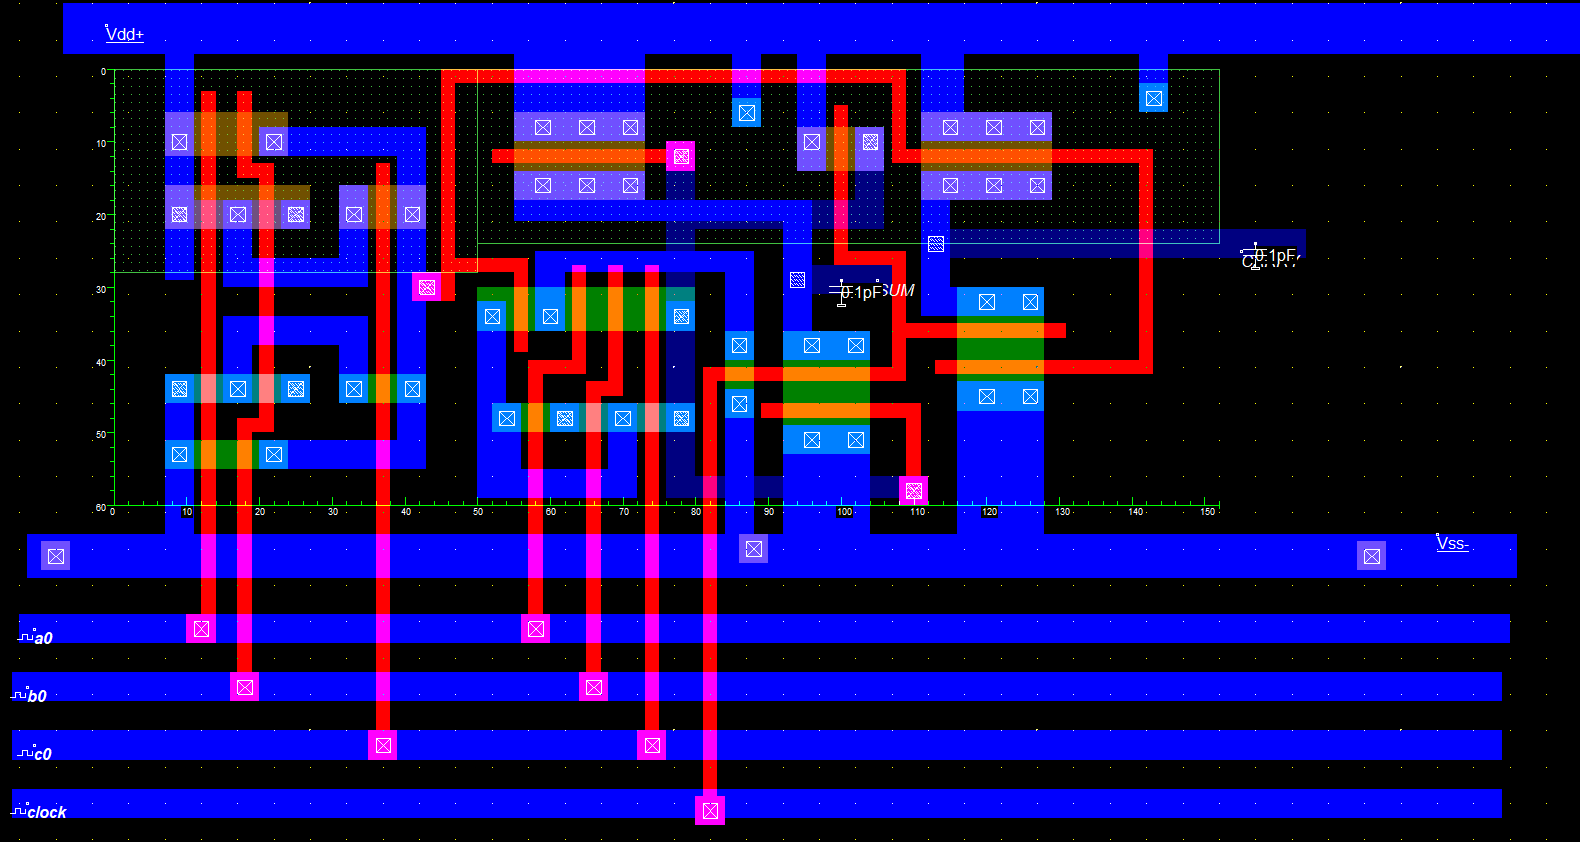
\includegraphics[scale=0.4]{Layout1_152x60}
Le dimensioni del circuito (escludendo le piste di alimentazione e quelle relative ai segnali) sono di $152 \lambda * 60 \lambda$, quindi coerenti con le specifiche assegnate.

\clearpage
\section{Simulazione}
Utilizzando le funzioni di simulazione del funzionamento del circuito di Microwind ho ottenuto i seguenti risultati\\
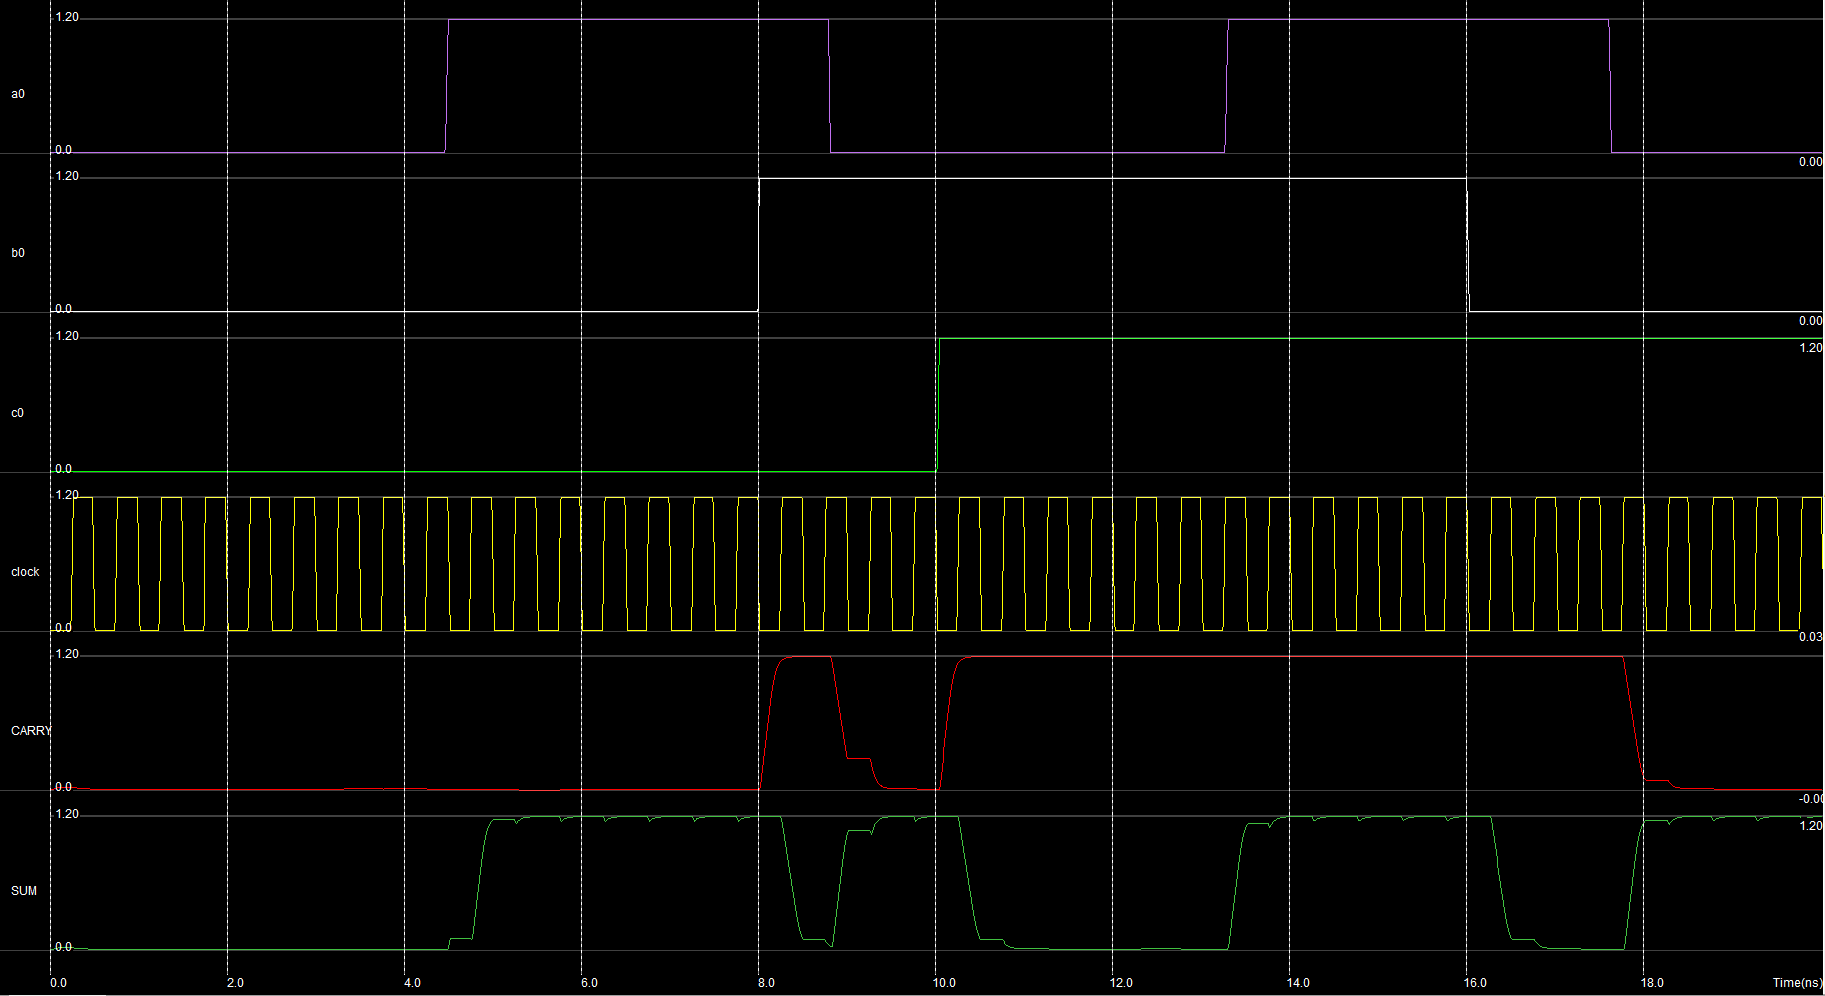
\includegraphics[width = 160mm, height = 150mm]{plot_microwind_layout1}
Dal punto di vista logico il circuito funziona correttamente, ma sono evidenti problemi di ritardi e raggiungimento del valore di uscita corretto, in particolare se si cambia il software di simulazione.
Utizzando Spice si ottengono i seguenti risultati:
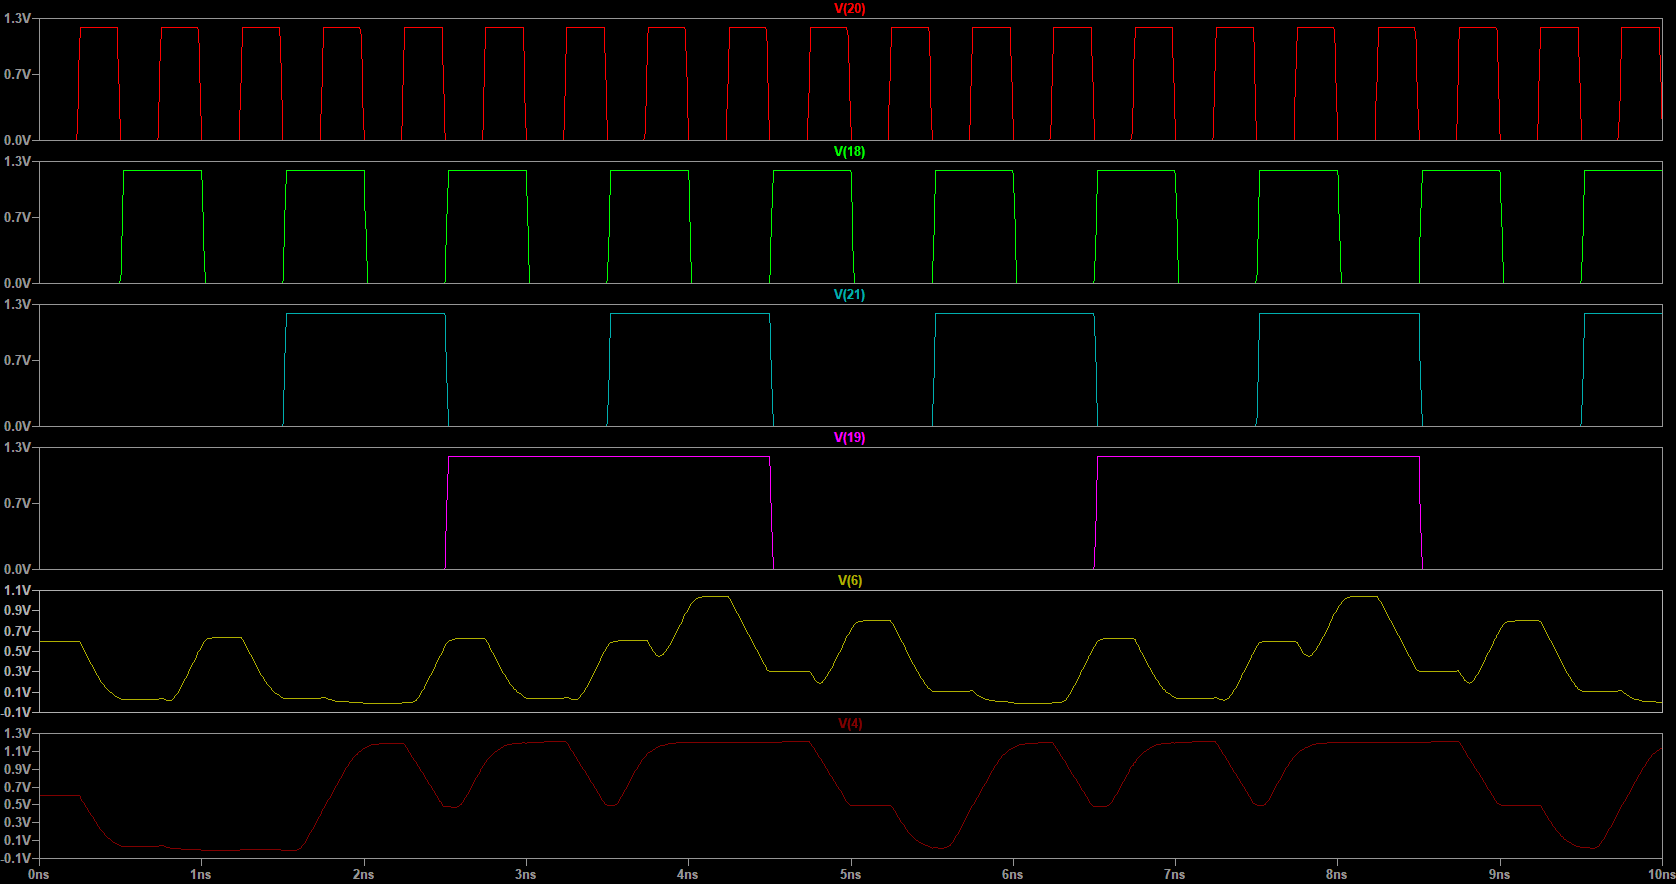
\includegraphics[width = 160mm, height = 150mm]{Vecchio}
I segnali nel grafico sono:
\begin{itemize}
\item Clock
\item A0
\item B0
\item C0
\item SUM
\item CARRY
\end{itemize}

Per risolvere questo problema è stato necessario ingrandire parte dei transistor iniziando dallo stadio di uscita. Seguendo la logica della fase di dimensionamento si è cercato un valore di W che permettesse al transistor di pilotare correttamente la capacità di uscita per poi ricalcolare la capacità di gate dei transistor ridimensionati e valutare le dimensioni più appropriate per gli stadi precedenti.\\
Poiché le differenze tra il valore atteso e quello ottenuto sono dovute alla differenza tra i modelli utilizzati (in fase di dimensionamento e dal simulatore), è stato necessario procedere empiricamente per ottenere dimensioni corrette dei componenti.

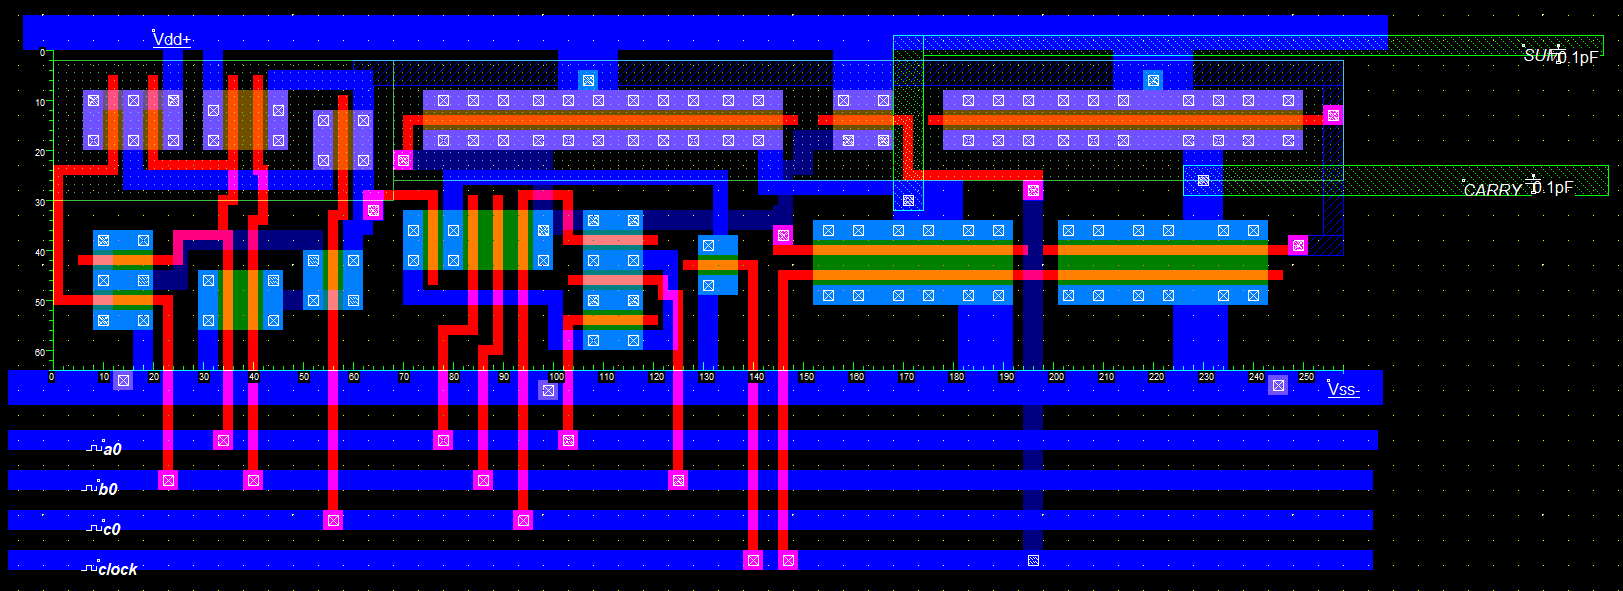
\includegraphics[scale = 0.35]{NuovoLayout_258x64}

Il layout così ottenuto ha delle dimensioni totali di  $258 \lambda * 64 \lambda$ (escludendo le piste di alimentazione, degli ingressi e quelle di uscita).

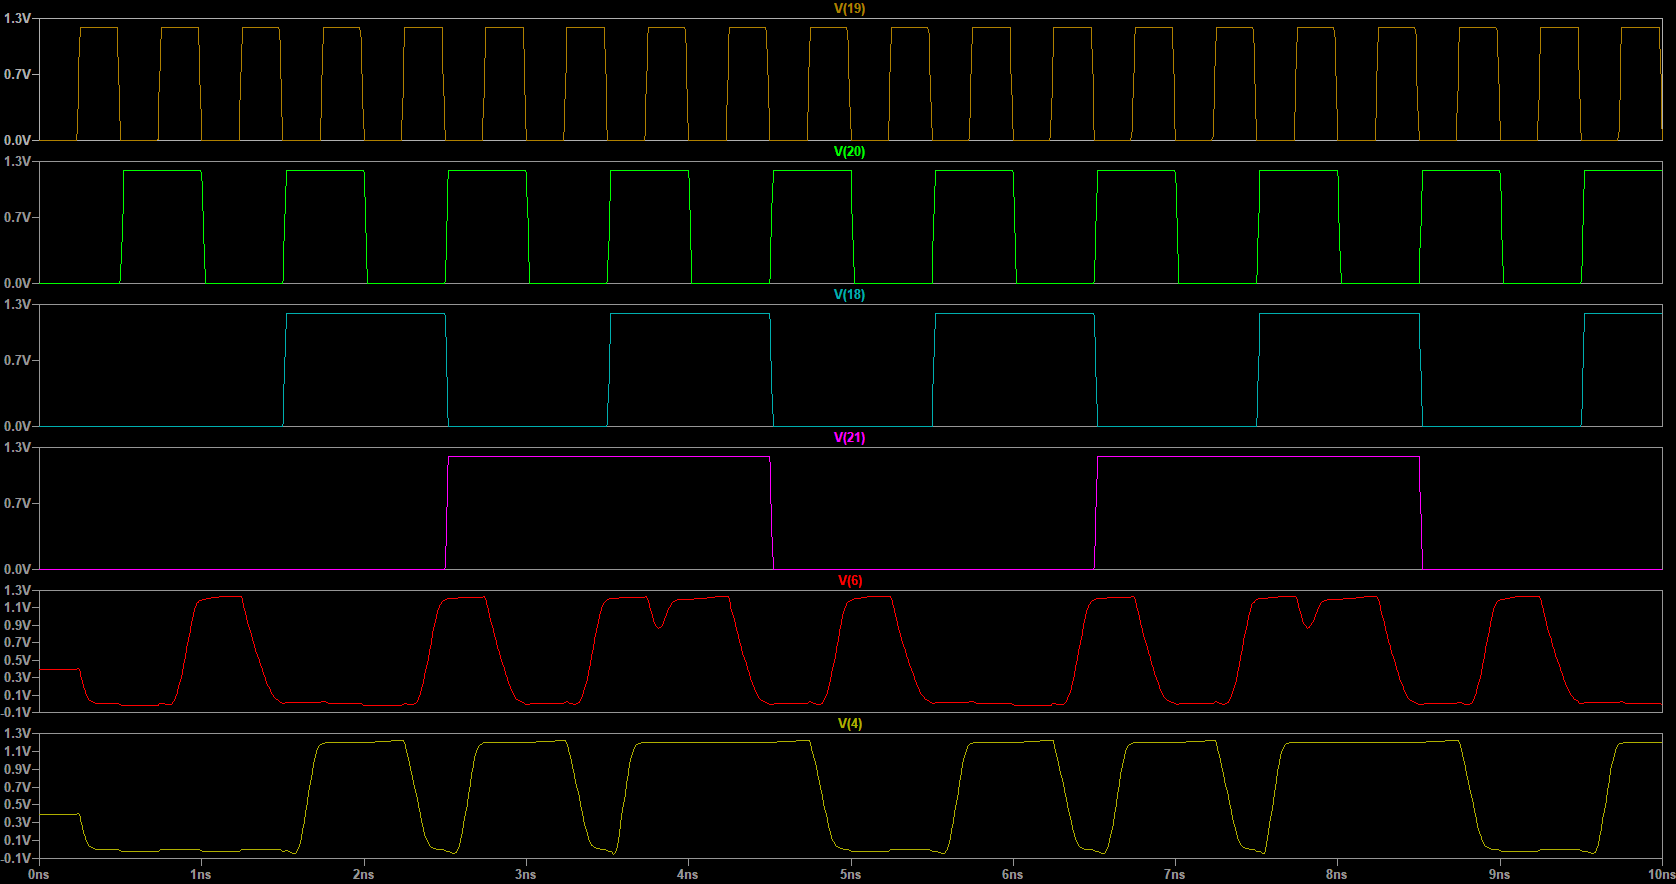
\includegraphics[width = 160mm, height = 140mm]{uscita_dimensioni_corrette}
I segnali nel grafico sono:
\begin{itemize}
\item Clock
\item A0
\item B0
\item C0
\item SUM
\item CARRY
\end{itemize}
Si può chiaramente osservare come le uscite raggiungano sempre il calore corretto e non si fermino a valori intermedi (come nel layout precedente).

\clearpage
\section{Analisi Potenza}

Per analizzare la potenza assorbita dal circuito si è sfruttato il software di simulazione Pspice, in particolare si è costruito il grafico considerando il prodotto tra la corrente e la tensione fornite dal generatore (cambiate di segno per convenzione dei generatori).

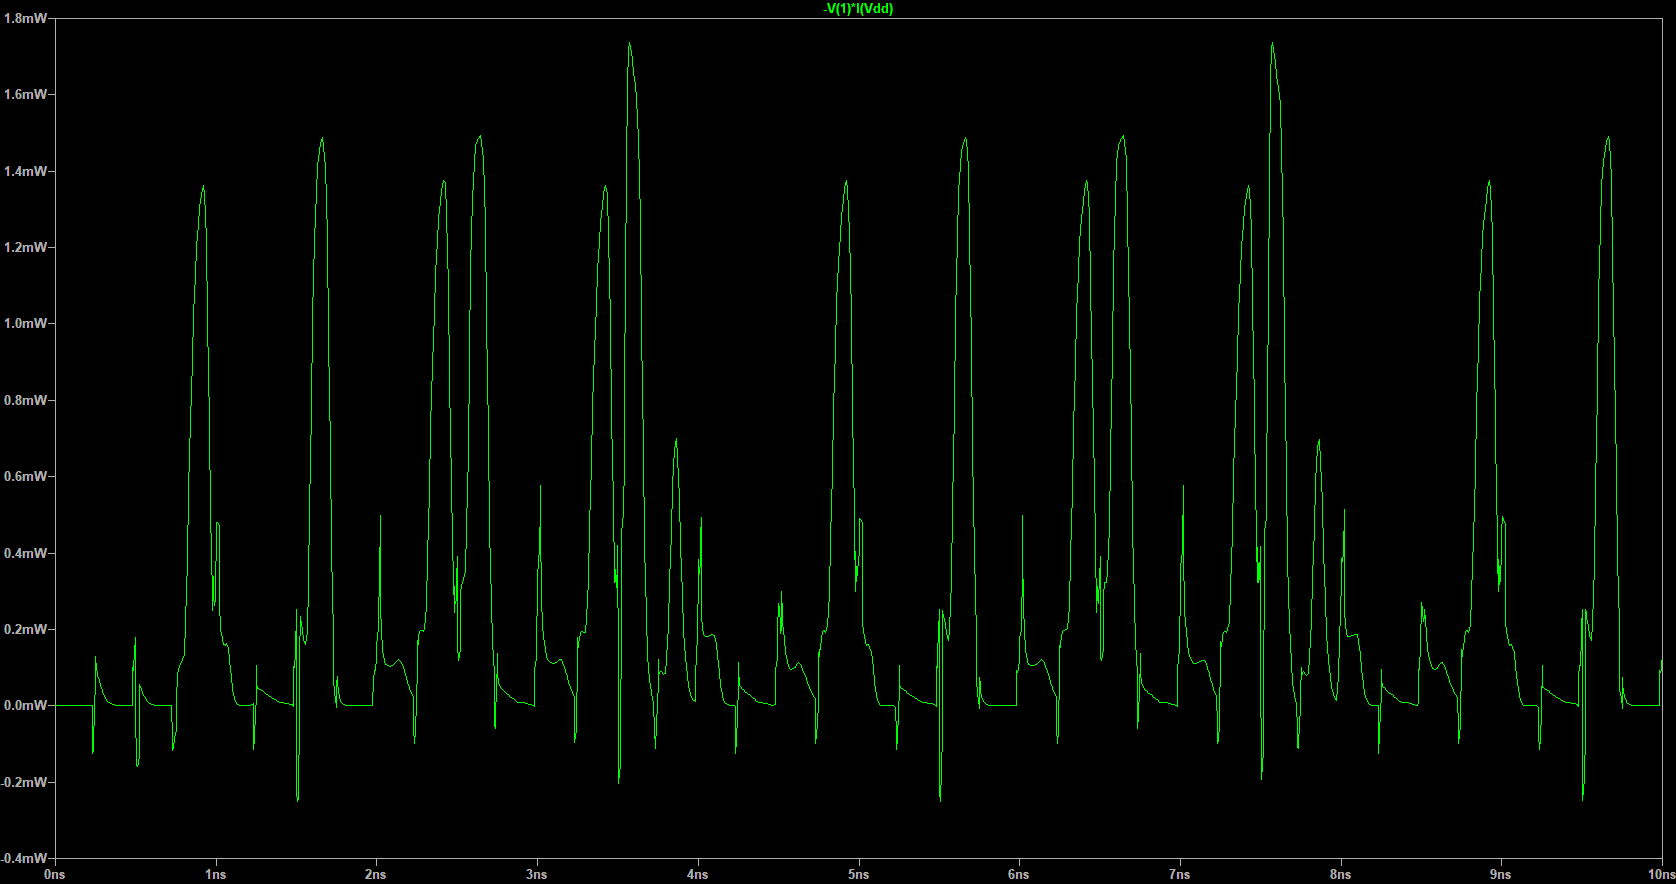
\includegraphics[scale = 0.35]{power}\\

Come si vede dal grafico la potenza fornita è quella necessaria per le transizioni (coerentemente con le caratteristiche dei transistor mos). Per avere un numero più significatori abbiamo quindi considerato la potenza media, ottenendo il seguente risultato.\\

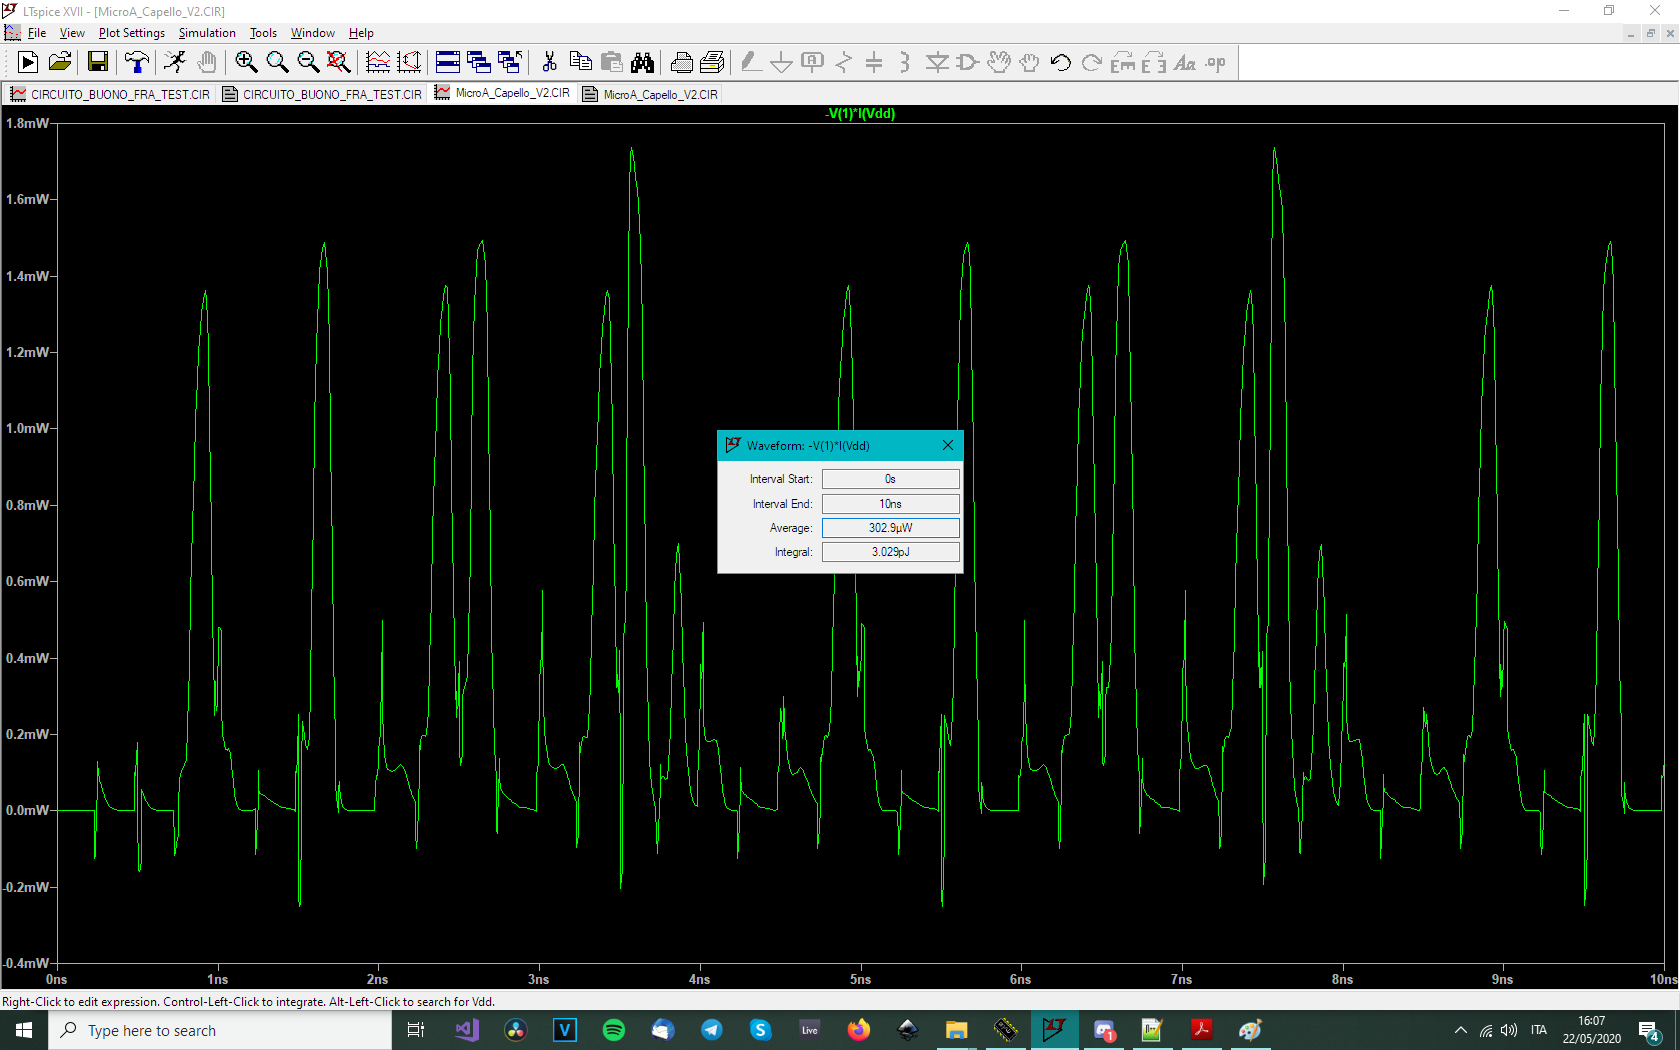
\includegraphics[scale = 1]{powerAvg}

\clearpage
\section{Conclusioni}
Il layour dell'adder a 1-bit realizzato ha le seguenti caratteristiche:
\begin{itemize}
\item Dimensioni: \quad $258 \lambda * 64 \lambda$
\item Potenza media: \quad $302.9 \mu W$
\end{itemize}

Non è stato realizzato l'adder a 4-bit poiché i ritardi nella generazione delle uscite di ogni adder a 1-bit avrebbero dato risultati privi di significato in uscita (poiché la richiesta era di un adder a 4-bit con ripple carry).

\section{Tool utilizzati}
Per lo svolgimento del progetto sono stati utilizzati i seguenti programmi:
\begin{itemize}
\item Microwind
\item LT Spice
\end{itemize}


\section{Bibliografia}
\begin{itemize}
\item Dispense e appunti del corso di Microelectronics
\item Jiren Yuan and Christer Svensson, “High-Speed CMOS Circuit Technique”.
\end{itemize}


\end{document}
